% backup | Intro to CS
% Add "% backup | [file name]" above (no quotes) to make file backup
\documentclass[12pt]{article}
% packages
\usepackage[paper=letterpaper,margin=2cm]{geometry}
\usepackage[skip=10pt plus1pt, indent=15pt]{parskip}
\usepackage{amsmath}
\usepackage{amssymb}
\usepackage{amsthm}
\usepackage{amsfonts}
\usepackage{graphics}
\usepackage{graphicx}
\usepackage{newtxtext, newtxmath}
\usepackage{titling}
\usepackage{setspace}
\usepackage[x11names]{xcolor}
\colorlet{shadecolor}{LavenderBlush3}
\usepackage{framed}
\usepackage[colorlinks=true]{hyperref}

% settings
\setlength{\droptitle}{-6em}

\begin{document}

\begin{titlepage}
    \begin{center}
        \vspace*{1cm}
        \Huge
        \textbf{Introduction to Computer Science}
        
        \vfill
        
        \begin{figure}[!ht]
            \centering
            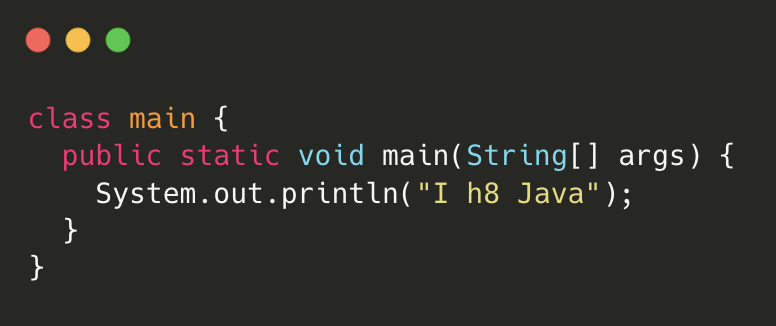
\includegraphics{misc/TITLEGRAPHIC.png}
        \end{figure}
        \vfill
        
        \small
        by Louis Meunier
        
        \href{https://notes.louismeunier.net}{\color{violet}{notes.louismeunier.net}}
        
    \end{center}
\end{titlepage}


{
  \hypersetup{linkcolor=violet}
  \tableofcontents
}

\newpage

\textit{Note that basic Java knowledge is assumed for these notes, so the first few chapters of this course are omitted for the sake of being concise.}

\section{UML Diagrams}

\textbf{UML Diagrams}: "Unified Modeling Language", a set of standards for creating diagrams to represented object-oriented systems - see figure \ref{fig:uml} for the basic layout, and figure \ref{fig:uml_example} for a basic example.

\begin{figure}[!ht]
    \centering
    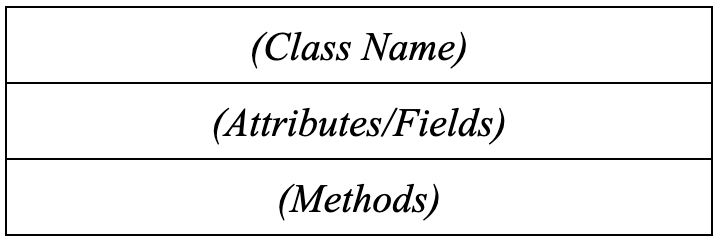
\includegraphics[width=8cm]{misc/uml.png}
    \caption{UML diagram layout}
    \label{fig:uml}
\end{figure}


\begin{itemize}
    \item A "+" before a field indicates public
    \item A "-" means private
    \item An underlined field means static
\end{itemize}

\begin{figure}[!ht]
    \centering
    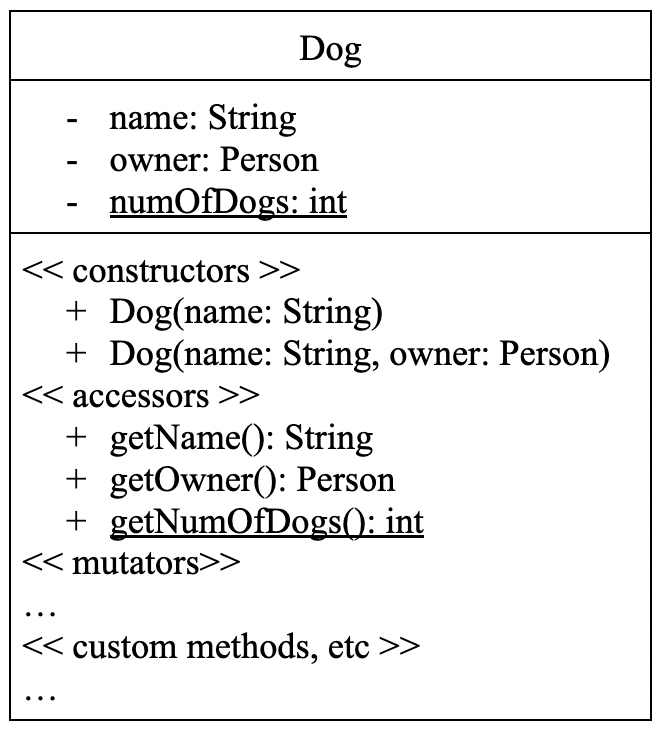
\includegraphics[width=7cm]{misc/uml_example.png}
    \caption{Example UML diagram}
    \label{fig:uml_example}
\end{figure}

\section{Basic Data Structures}
\subsection{Singly Linked Lists}
\textbf{Single Linked List}: an object made up nodes with both links to the next item in the list, as well as a reference to an element. Figure \ref{fig:singlylinked} demonstrates this well.

\begin{figure}[!ht]
    \centering
    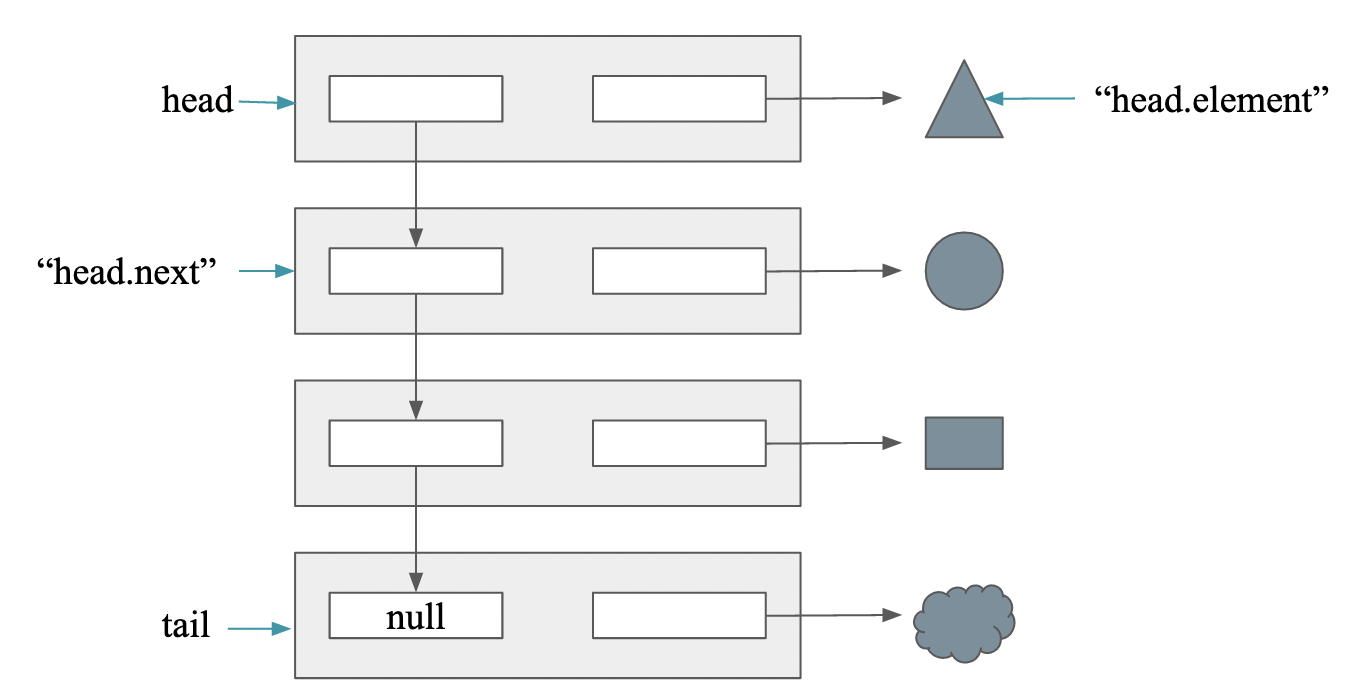
\includegraphics[width=12cm]{misc/singlylinkedlist.png}
    \caption{Singly Linked List}
    \label{fig:singlylinked}
\end{figure}

An implementation of a Linked List object should include both a head (first) and tail (last) node, as well as a field representing its size. Each node within the list should also include both an "element" field and a reference to the next node in the list.  

Appropriate methods that should also be added to the list include \textit{addFirst()}, \textit{removeFirst()}, \textit{addLast()}, and \textit{removeLast()}. It should be noted that all these methods are able to be implemented in O(1) time complexity \textit{except} removeLast(), which is possible in O(N) time. Hopefully this should be intuitive, as for this last method, you must iterate over the entire list until the second-to-last node, which must then be updated to set the last "element.next" to "null".

\subsection{Doubly Linked Lists}
\textbf{Doubly Linked Lists}: have all the same properties as singly linked lists, but also have a reference to the previous element in the list: see figure \ref{fig:doublylinked}.

\begin{figure}[!ht]
    \centering
    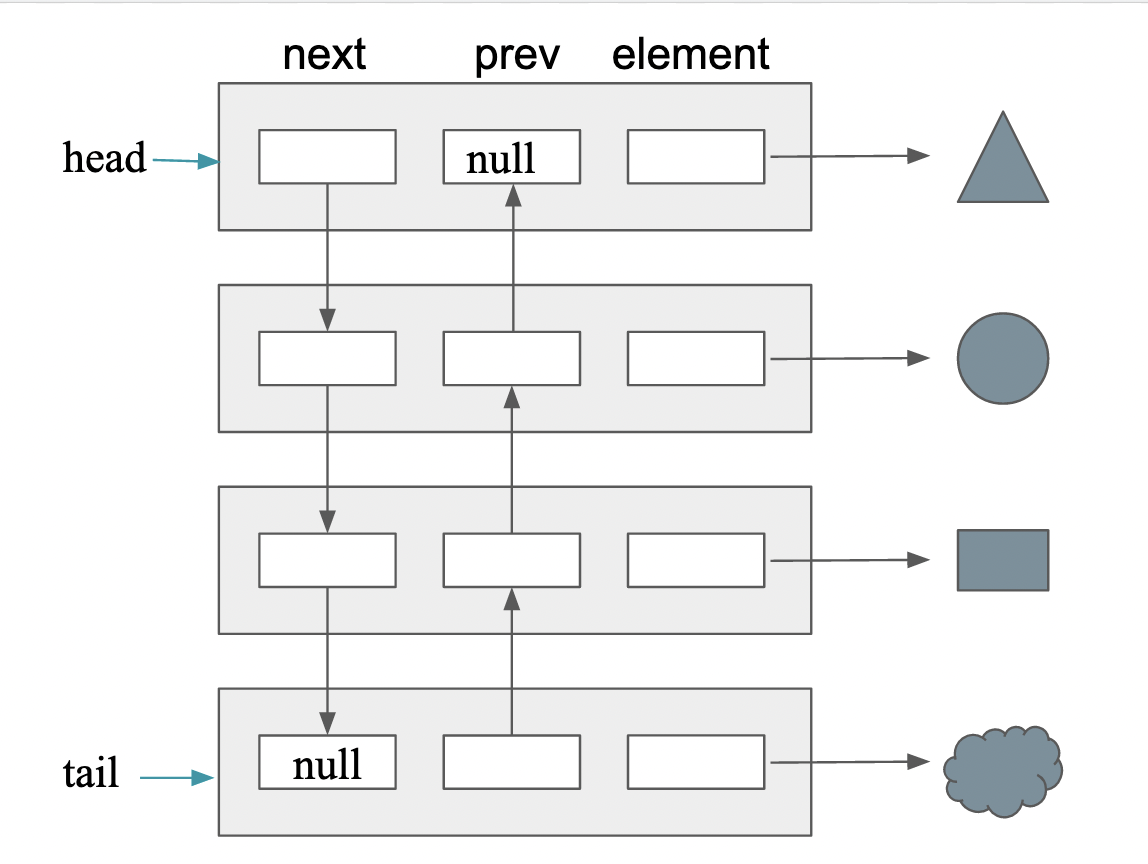
\includegraphics[width=11cm]{misc/doublylinkedlist.png}
    \caption{Doubly Linked List}
    \label{fig:doublylinked}
\end{figure}

The 4 methods mentioned above for a singly linked list also apply to a doubly linked list, except the method \textit{removeLast()} can be implemented in O(1). This should be intuitive: as you can access the second-to-last node and set its "next" to "null" in constant time by simply accessing "tail.prev".

It should be noted that even though the \textit{time} complexity is better, the \textit{space} complexity is worse; each node in a doubly-linked list actually contains 3 objects, while each node in a singly-linked list contains 2 (plus the object representing the list itself).

\subsection{Stacks}

Stacks, as the name implies, are a data structure that follows the \textit{LIFO} (Last In, First Out) principle. This means that the last element added to the stack is the first element removed from the stack.

\subsection{Queues}

Somewhat inverse to stacks, queues act like lines: the first element added to the queue is the first element removed from the queue. This is known as the \textit{FIFO} (First In, First Out) principle. This can be implemented in a number of ways, but one popular method is to use a circular array, which, as more elements are added, automatically expands.

\section{Sorting}
Sorting algorithms are one of the most common algorithms used in programming, and their efficiency is important to understand. While some are clearly better than others in all circumstances, some are better when inputs are of a certain type/etc..

\subsection{$O(n^2)$: Quadratic Sorting}
All of these algorithms sort elements in $O(n^2)$ time; ie, the time complexity is proportional to the size of the array squared.

\subsubsection{Bubble Sort}
Iterate through a list, and swap adjacent elements if they are in the wrong order. This is perhaps the "simplest" algorithm.

\textit{Pseudocode implementation:}

\begin{verbatim}
    sorted = false
    i = 0
    while (!sorted) {
        sorted = true
        for j from 0 to list.length - i - 2 {
            if (list[j] > list[j+1]) {
                swap(list[j], list[j+1])
                sorted = false
            }
        }
        i++
    }
\end{verbatim}

For an array $[5,1,4,2,8]$, the following shows the algorithm during the first iteration:

\begin{itemize}
    \item $[1,5,4,2,8]$
    \item $[1,4,5,2,8]$
    \item $[1,4,2,5,8]$
    \item $[1,4,2,5,8]$
    \item etc..
\end{itemize}

This continues logically, until the array is sorted. It is important to realize that, when determining how many iterations it takes to sort the array, you have to take into account the last iteration after the array is sorted that the algorithm must take to ensure the array is actually sorted.

\subsubsection{Selection Sort}
\begin{itemize}
    \item Consider the list in two parts: one that is sorted at the beginning, and one that is unsorted at the end.
    \item Select the smallest element in the unsorted part of the list
    \item Swap this element with the element in the initial position of the unsorted part
    \item Change the sorted/unsorted division in the array
\end{itemize}

\textit{Pseudocode:}

\begin{verbatim}
    // repeat until list is all sorted (~N)
    for delim from 0 to N - 2 {
        // find the index of the min element in the unsorted section of the array
        min = delim
        for i from delim + 1 to N - 1 {
            if (list[i] < list[min]) {
                min = i
            }
        }
        // swap the min element with the first element 
        // of the unsorted section of the array
        if (min != delim) {
            swap(list[min], list[delim])
        }
    }
\end{verbatim}

\newcommand{\blue}[1]{\textcolor{violet}{#1}}

The following steps represent how this algorithm roughly works, where $\blue{|}$ represents the delimiter between sorted (toward the beginning) and unsorted (toward the end):

\begin{itemize}
    \item $[\blue{|}5,1,7,2]$
    \item $[1\blue{|}5,7,2]$
    \item $[1,2\blue{|}7,5]$
    \item $[1,2,5\blue{|}7]$
    \item $[1,2,5,7\blue{|}]$
\end{itemize}

\subsubsection{Insertion Sort}
\begin{itemize}
    \item Consider the list in two parts: one that is sorted at the beginning, and one that is unsorted at the end.
    \item Select the first element of the unsorted part of the list
    \item Insert this element into the correct position of the sorted part of the list
    \item Change where the array is delimited between sorted/unsorted
\end{itemize}

\textit{Pseudocode:}

\begin{verbatim}
    // repeat until list is sorted (~N)
    for i from 0 to N - 1 {
        // find where the next element in the unsorted portion 
        // should be inserted into the sorted part of the list and make space for it
        element = list[i]
        k = i
        while (k > 0 && element < list[k-1]) {
            list[k] = list[k - 1]
            k--
        }
        // insert the element into the sorted part of the list 
        list[k] = element
    }
\end{verbatim}

Example steps:

\begin{itemize}
    \item $[\blue{|}5,1,7,2]$
    \item $[5\blue{|}1,7,2]$
    \item $[1,5\blue{|}7,2]$
    \item $[1,5,7\blue{|}2]$
    \item $[1,2,5,7\blue{|}]$
\end{itemize}

\section{Asymptotic Notation}

This section will cover a variety of notations used to analyze a particular function's efficiency.

\subsection{\texorpdfstring{Big-$O$ Notation}{TEXT}}

Formally, given a function $g(n)$, $O(g(n))$ is defined as:

\begin{equation}
    O(g(n)) = \{f(n): \exists c, n_0 \in \mathbb{N} \text{ s.t. } 0 \leq f(n) \leq c \cdot g(n) \text{ for all } n \geq n_0\}
\end{equation}

In other words, $O(g(n))$ is the set of functions that are bounded above by a constant multiple of $g(n)$. \textit{This is where the term asymptotic comes from, as the function is asymptotically bounded by $g(n)$}.

Graphically, see figure \ref{fig:bigO}.

% insert graph

To make more sense of this, take the function $5n+70$. 

\begin{proof}
    Our goal is to find some $c$ such that $cn$ upper bounds $5n+70$ when $n\geq n_0$; in others words, $5n+70 \leq cn, n \geq n_0$.

    Let's pick some $n_0$ that makes the upper bound easy to compute: $n_0 = 1$. 
    
    We can use our $n_0$ to see if $c$ exists:

    \begin{equation}
        \begin{split}
            5n + 70 \leq cn, n \geq 1 \\
            5n + 70 \leq 75n, n \geq 1 \\
            \therefore c = 75\\
        \end{split}
    \end{equation}

    Thus, there exists a $n_0$ and corresponding $c$ such that $5n+70 \leq cn, n \geq n_0$, and therefore $5n+70 \in O(n)$. Clearly, we could have picked any $n_0$ and calculated the corresponding $c$, and this would have held.
\end{proof}

Note that because $O(n)$ is an upper bound, it therefore represents the worst case scenario for a function. Specifically, it represents a tight upper bound, since if a function is upper bounded by $O(n^2)$, it is also upper bounded by $O(n^3), O(n^4),$ etc.

\subsection{Properties of Asymptotic Functions}

\begin{itemize}
    \item \textbf{Scaling:} For all constant $a>0$, if $f(n)$ is $O(g(n))$, then $af(n)$ is also $O(g(n))$.
    \item \textbf{Sum Rule:} If $f_1(n)$ is $O(g(n))$ and $f_2(n)$ is $O(h(n))$, then $f_1(n) + f_2(n)$ is $O(g(n) + h(n))$.
    \item \textbf{Product Rule:} If $f_1(n)$ is $O(g(n))$ and $f_2(n)$ is $O(h(n))$, then $f_1(n) \cdot f_2(n)$ is $O(g(n) \cdot h(n))$.
    \item \textbf{Transitivity Rule:} If $f(n)$ is $O(g(n))$ and $g(n)$ is $O(h(n))$, then $f(n)$ is $O(h(n))$.
\end{itemize}

\subsection{\texorpdfstring{Big-$\Omega$ Notation}{TEXT}}

While Big-$O$ notation is concerned with the \textit{upper} bound of a function, Big-$\Omega$ notation is concerned with the \textit{lower} bound of a function. More specifically, we can say that some function $f(n)$ is asymptotically lower bounded by $g(n)$ if there exists some $n_0$ such that for all $n$ greater than or equal to $n_0$, then $f(n) \geq g(n)$.

More formally, we can say:

\begin{equation}
    \begin{split}
        \Omega(g(n)) = \{f(n): \exists c, n_0 \in \mathbb{N}, c, n_0 > 0, \text{ s.t. } f(n) \geq c \cdot g(n) \text{ for all } n \geq n_0\}
    \end{split}
\end{equation}

Notice that this is almost identical to the definition of Big-$O$ notation, except that the inequality is flipped.

Say we want to prove that the lower bound of $f(n) = \frac{n(n-1)}{2}$ is lower bounded by $g(n) = n^2$. We can take $c=\frac{1}{4}$, and say:

\begin{equation}
    \begin{split}
        \frac{n(n-1)}{2} \geq cn^2\\
        \frac{n(n-1)}{2} \geq \frac{n^2}{4}\\
        \frac{n^2-n}{2} \geq \frac{n^2}{4}\\
        2n^2-2n \geq n^2\\
        n^2 \geq 2n\\
        n \geq 2\\
        \therefore n_0 = 2
    \end{split}
\end{equation}

Thus, an $n_0$ and $c$ exist for this inequality to be true, so $f(n) \geq cn^2, n \geq n_0$, and therefore $f(n) \in \Omega(n^2)$.

\subsection{\texorpdfstring{Big-$\Theta$ Notation}{TEXT}}

While Big-$O$ described worst performance (upper bound) and Big-$\Omega$ described best performance (lower bound), Big-$\Theta$ describes a tight bound; in other words, it describes both of the previous sets. More formally, we can say that some function $f(n)$ is $\Theta(g(n))$ if there exist three positive constants $n_0, c_1, c_2$ such that for all $n\geq n_0$:

\begin{equation}
    c_1g(n) \leq f(n) \leq c_2g(n)
\end{equation}

Notice that this definition is simply combining Big-$O$ and Big-$\Omega$.

Also note that Big-$\Theta$ does not always exist; we can say:

\begin{equation}
    f(n) = \Theta(g(n)) \iff f(n) \in O(g(n)) \cap \Omega(g(n))
\end{equation}

\section{Induction}

Induction, while more generally used in math, is helpful in a variety of computer science applications (such as proving run times, etc.). Induction is a method of proving a statement about a set of numbers, and is based on the idea that if a statement is true for a number, it is true for all numbers greater than that number.

Generally, you are given a statement to prove (say, $f(n)\geq g(n)$), and a base condition that said statement must be proven for (say, $n\geq 1$). You can then prove the statement by showing that it is true for the base condition, and then showing that if it is true for $n$, it is true for $n+1$. We can break this down into three steps:

\begin{itemize}
    \item \textbf{Base Clause}
    \item \textbf{Inductive Clause}
    \item \textbf{Final Clause}
\end{itemize}

Say, for instance, you'd like to prove that $1+2+3+...+(n-1)+n = \frac{n(n+1)}{2}$ for all natural numbers $n\geq 1$. To prove this inductively, we follow the outline above and say:

\begin{itemize}
    \item \textbf{Base Clause:}
    
    Does this hold for the base clause, ie $n = 1$? We can check:
    
    \[
        1 = \frac{1*(1+1)}{2} = 1
    \]

    Since this holds true for our base case (note that this came from the original question...) we can then move on to\dots

    \item \textbf{Inductive Clause:}
    
    Assume that our statement holds true for $k$; can we prove it holds for $k+1$? To consider why this step makes logical sense, imagine $k=1$, our base clause. We've proved this is true, so we can then see if $k+1$ is true. Technically, we could continue checking our statement this way until infinity, but instead, if we simply prove it generally using an arbitrary $k$, we can then say that it holds for all $k$.

    For this specific situation, we can say (using the assumption that $k$ satisfies our statement):

    \[
      1 + 2 + ... + k = \frac{k(k+1)}{2}  
    \]

    We can check if $k+1$ holds using this assumption:

\[
    \textcolor{red}{1 + 2 + ... + k }+ (k+1) = \frac{(k+1)(k+1+1)}{2}
\]
The left side of this operation is simply our original  assumption (in red) plus $k+1$, so we can rewrite:


\[
   \textcolor{red}{\frac{k(k+1)}{2}} +k+1= \frac{(k+1)(k+2)}{2}
\]

This simplifies to the same equation on either side, and thus we can say that our statement is true inductively

\end{itemize}

\section{Recursion}
\end{document}